\chapter[Introducción]{Introducción}
\label{Chap1}

Las Naciones Unidas definen el cambio climático como el conjunto de \textit{"cambios a largo plazo de las temperaturas y los patrones climáticos"} \cite{UNWeb}. Estos pueden ocurrir de forma natural cada cierto tiempo como tenemos sabido, ya sea debido a erupciones volcánicas, fluctuaciones de la radiación solar e, incluso, variaciones en la órbita terrestre, llegando a causar climatologías extremas como pueden ser las glaciaciones. Actualmente, a este proceso se le debe añadir como causa la actividad humana, alterando y agravando los efectos, siendo los principales causantes la contaminación, sobre-población y la deforestación.\newline
\newline
Partiendo desde principios de la revoluciona industrial a mediados del siglo XVIII, el efecto de la actividad humana como causa de estos cambios ha ido en aumento, siendo desde el siglo XIX hasta llegar a pleno siglo XXI la principal causa del cambio climático. Debido al uso extendido de combustibles fósiles tales como el carbón, petroleo y el gas, formando las principales fuentes de energía durante muchos años.\ref{fig:ej16}\newline
\newline
La quema de estos produce los llamados gases de efecto invernadero, principalmente dióxido de carbono y metano. Estos gases impiden la correcta liberación de la radiación irradiada por el suelo al ser calentado por el sol, absorbiendo parte de esta y liberándola nuevamente hacia la tierra, aumentando la temperatura terrestre.\ref{fig:ej17}

\begin{figure} [H]
	\centering
	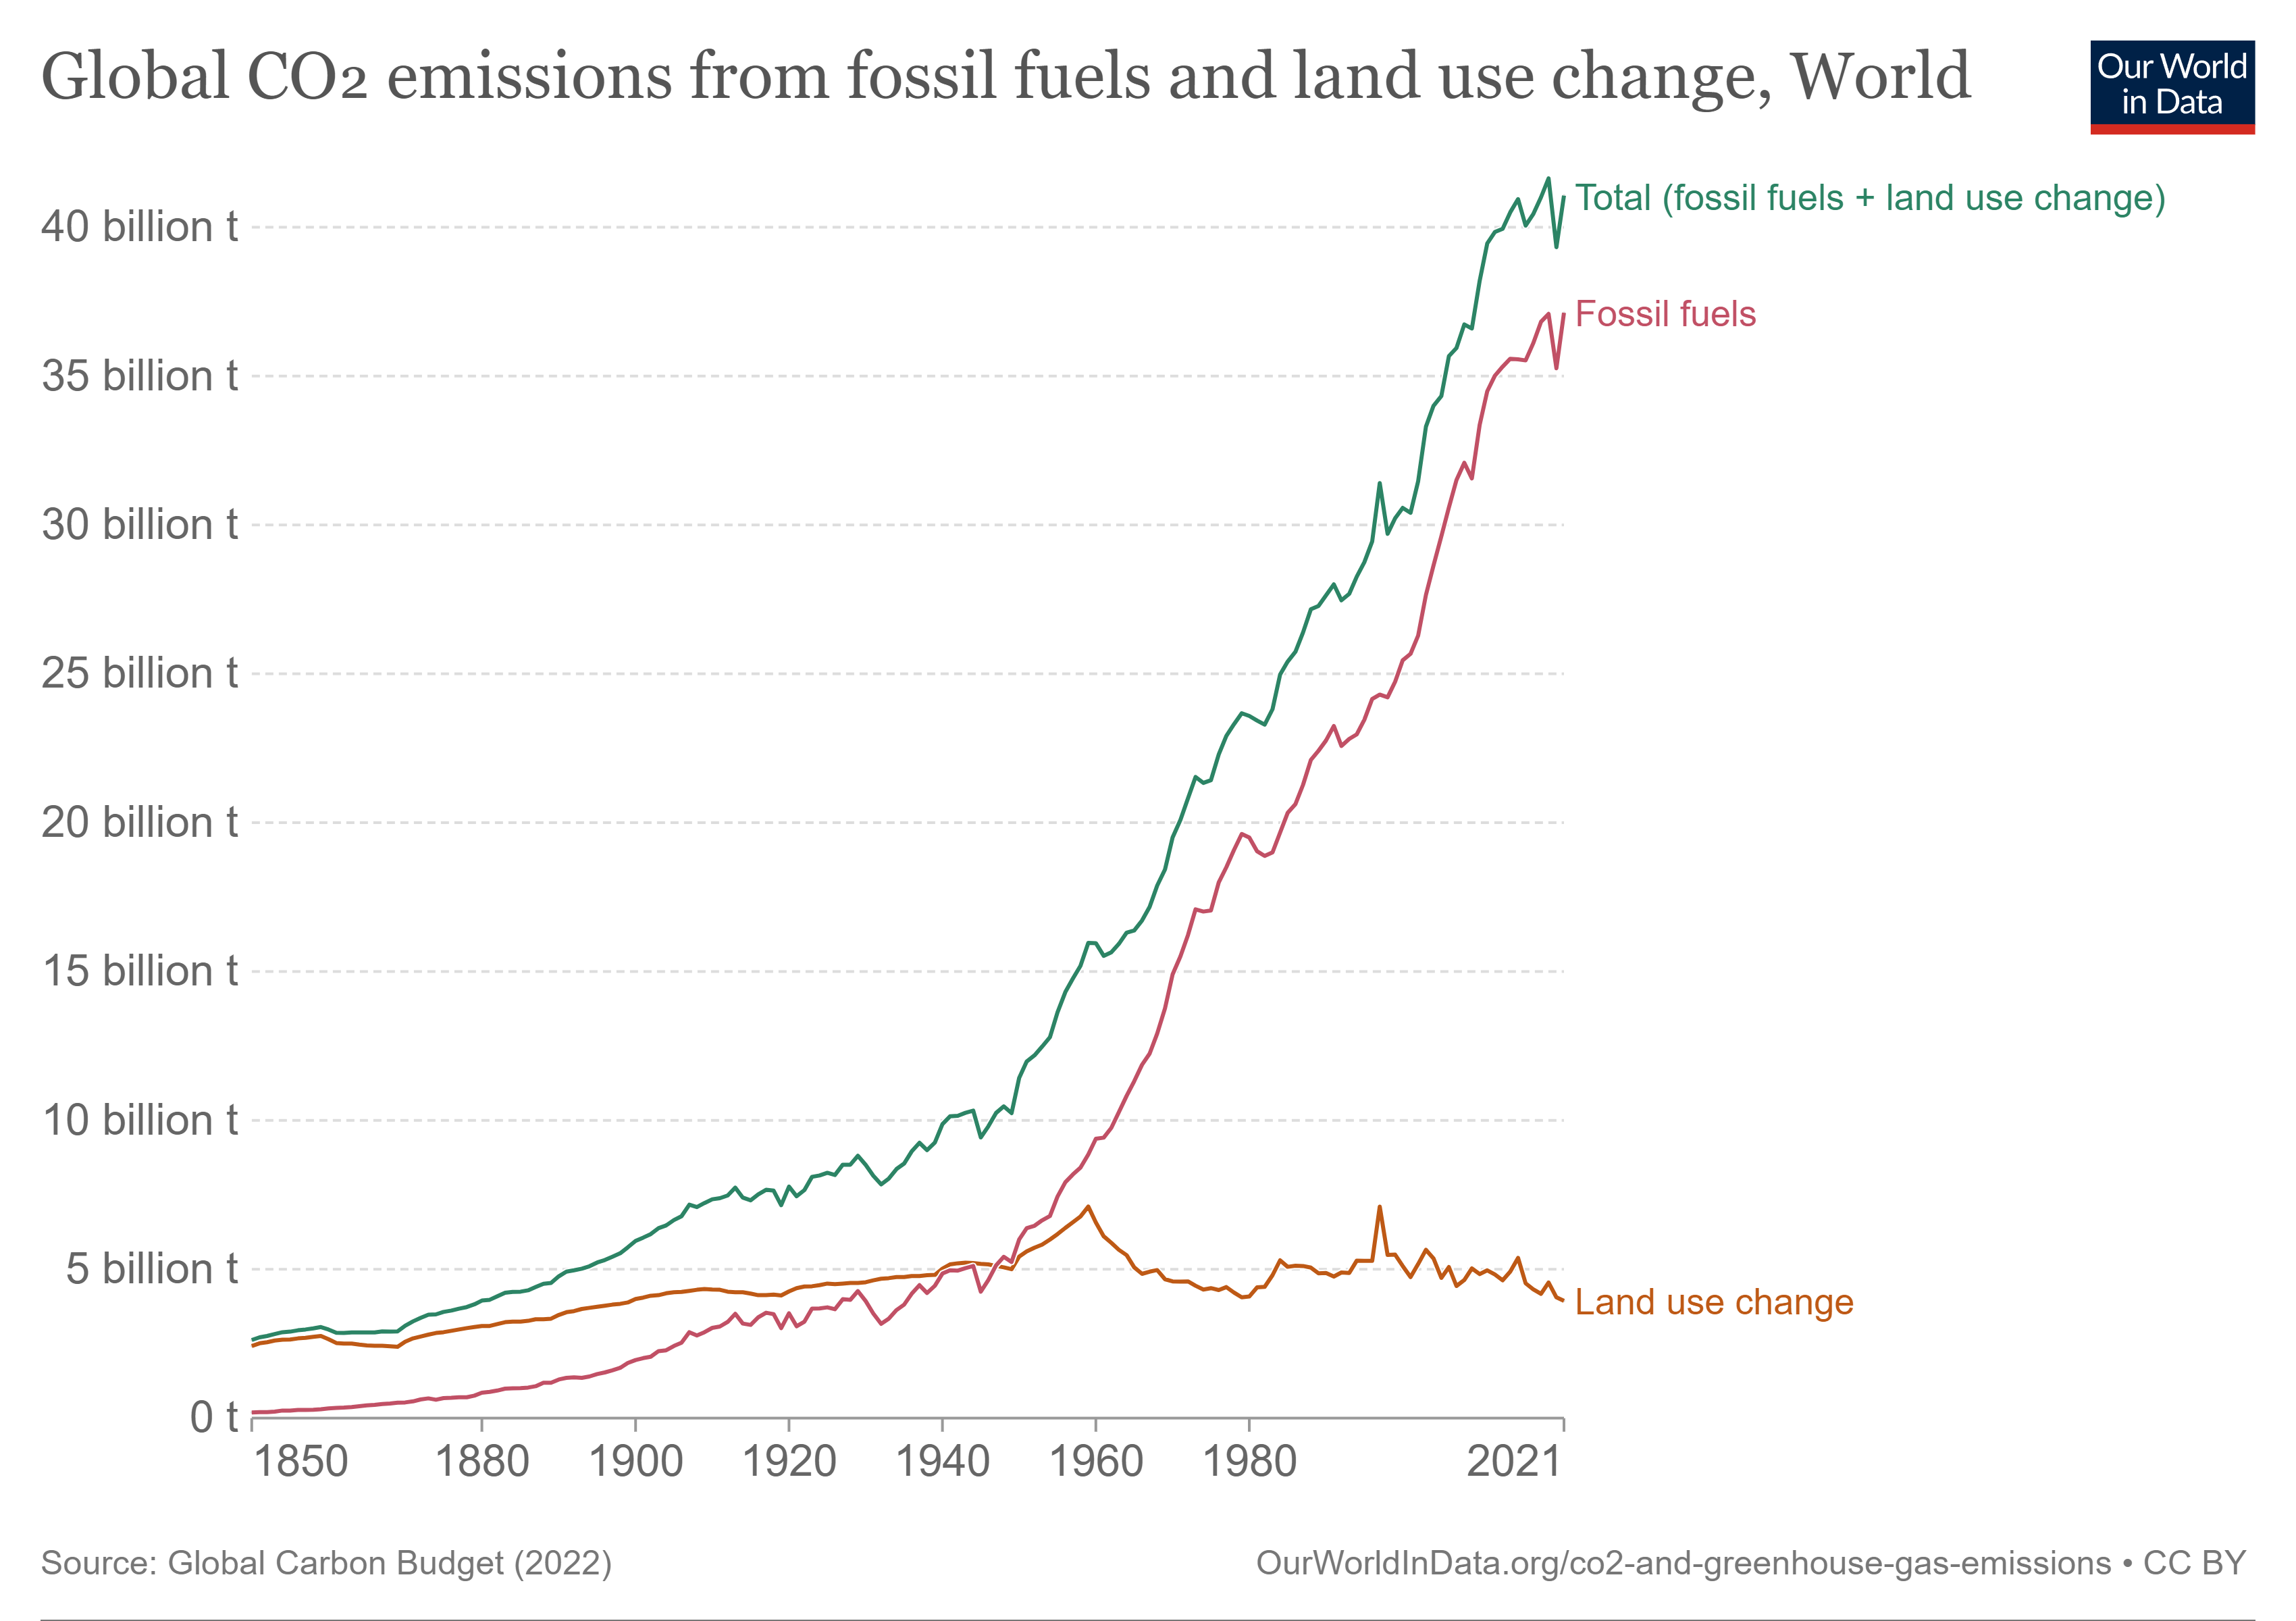
\includegraphics[width=0.7\textwidth]{fig/global-co2-fossil-plus-land-use.png}
	\caption[Emisiones globales de CO2]{Emisiones globales de CO2 \footnotemark}
	\label{fig:ej16}
\end{figure}
\footnotetext{\url{https://ourworldindata.org/co2-emissions}}

\begin{figure} [H]
	\centering
	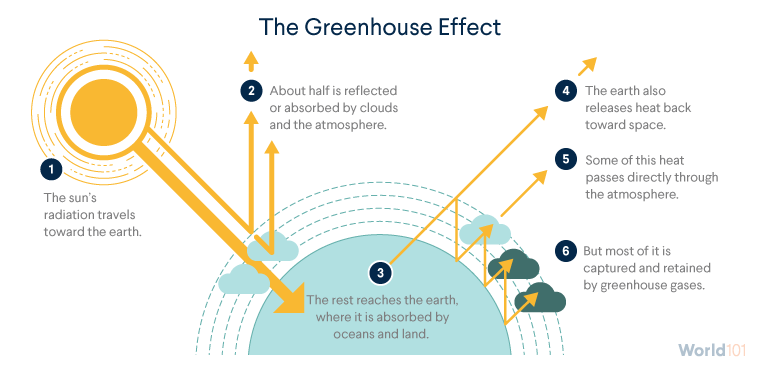
\includegraphics[width=0.7\textwidth]{fig/climate-change_greenhouse-effect_steps.png}
	\caption[Efecto invernadero]{Efecto invernadero \footnotemark}
	\label{fig:ej17}
\end{figure}
\footnotetext{\url{https://world101.cfr.org/global-era-issues/climate-change/greenhouse-effect}}

El aumento de emisiones de estos gases, a fomentado una crecida sustancial en la velocidad de elevación de la temperatura terrestre. Llegando a medirse un aumento regional de, entre 0.8\textdegree C hasta 2\textdegree C en altas latitudes, estimando un aumento en la media global de 1.1\textdegree C en comparación con finales del siglo XIX. \cite{ruddiman2003anthropogenic}\newline
\newline
Década tras década las temperaturas han ido aumentando, llegando a un punto en el que prácticamente anualmente se baten récords de temperatura máximas por todo el globo. \ref{fig:ej18} \cite{NCEIWeb}

\begin{figure} [H]
	\centering
	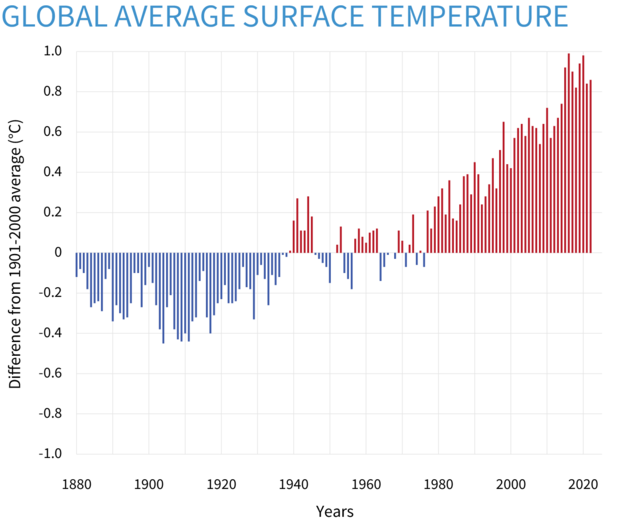
\includegraphics[width=0.7\textwidth]{fig/ClimateDashboard-global-surface-temperature-graph-20230118-1400px.png}
	\caption[Media de aumento de temperatura global entre 1901-2000]{Media de aumento de temperatura global entre 1901-2000 \footnotemark}
	\label{fig:ej18}
\end{figure}
\footnotetext{\url{https://www.climate.gov/news-features/understanding-climate/climate-change-global-temperature}}

El efecto causado por la subida de la temperatura tiene múltiples efectos adversos, entre ellos, la subida del nivel marino, reduciendo e inundando zonas costeras, la desertificación de zonas actualmente áridas y la alteración del comportamiento de especies tanto animales como vegetales, llegando a suponer una reducción sobre la población en multitud de especies \cite{arnell2019global} \cite{new2011four}. Es por eso que múltiples países son ya los que optan por comprometerse a alcanzar una cota de emisiones cero para 2050, tratando de reducir las emisiones globales a la mitad cara 2030 con el fin de mantener el aumento de la temperatura media por debajo de 1.5\textdegree C, estimando esta como un punto reflexivo a la hora de controlar el impacto climático, manteniendo un clima habitable.





\section{Antigua intro al parecer inutil :v}
Los últimos 15-20 años la Unión Europea ha realizado un gran esfuerzo en promover políticas de datos abiertos en realización a la información generada y monitorizada por los estados miembros. El objetivo de esta política es acercar estos datos a la población para tener un mayor control territorial y medio ambiental. El gobierno de Navarra y de España contribuyen a la oferta de datos abiertos publicando mediante diferentes organismos como el geoportal (\url{https://geoportal.navarra.es/es/idena}) en Navarra o los datos o el sistema automático de información publicada por las diferentes confederaciones hidrográficas en España.\newline
\newline
El objetivo de este trabajo es crear una plataforma habilitada en técnicas de scraping, centralizando la información proveniente de diferentes fuentes para una posible futura predicción y aviso de inundaciones mediante los datos pluviométricos obtenidos de los ríos de Navarra.\newline
\newline
La plataforma se dividirá en dos apartados, la obtención de los datos y el almacenamiento de estos. Para ello se harán uso de dos máquinas virtuales comunicándose entre si. Aunque hacer uso de una única máquina no solo es viable si no más sencillo, disponer de ellas, no solo aparta la plataforma de un diseño centralizado mas vulnerable, ademas, a nivel de proyecto, proporciona un mayor grado de complejidad, necesitando configurar la comunicación por red de estas.\newline
\newline
La primera máquina sera la encargada del almacenamiento de los datos, proporcionando una base de datos en PostGreSQL. Esta recibirá los datos de la segunda máquina, encargada de la obtención de estos.\newline
\newline
Como se ha mencionado, la plataforma busca centralizar los datos proporcionados en las distintas webs, tanto fluviales como pluviométricos, creando un punto de acceso global para su posterior uso. Es por eso que la segunda máquina dispone de una plataforma automática de obtención de datos mediante scraping web que, junto a una API en Django posibilita el envío de los datos a la base de datos.\newline
\newline
Esta plataforma, realizada usando el Framework de Python Scrapy para el apartado de obtención de datos y, Cron para la automatización, ejecuta los scripts de forma regular en intervalos de tiempo predefinidos para cada web, con el fin de no generar más trafico web del realmente necesario.\newline
\newline
En este proyecto se ha pretendido crear una plataforma lo más modular posible, ya sea por el uso de múltiples máquinas virtuales, como por los distintos apartados que la forman e, incluso en la forma de codificarla. Intenta ser lo más intuitiva posible a la hora de poder realizar cambios sobre esta, diferenciando claramente cada elemento.\newline
\newline
Centrado en técnicas de scraping web, este proyecto esta limitado por los datos ofrecidos de forma abierta en la web, siendo su punto débil, aquel del cual no disponemos control alguno. A día de hoy, la plataforma dispone de cuatro fuentes distintas de las cuales obtener datos, pero esta comprometida a que se mantengan invariables en el tiempo. Es por esto, que en un proyecto así necesariamente se debe valorar la búsqueda de datos de forma activa. No solo para su mantenimiento a largo plazo sino como forma de extender su alcance.\newline
\newline